%---- MSE Presentation Sonova ------
%---- Begin editing after PREAMBLE END at line 77------
%---- Created by: Matthias Meyer 2022 --
%---- matthias.meyer@sonova.com -----

\documentclass[xcolor=dvipsnames,envcountsect]{beamer}

%------------------------------------------------
%------------------------------------------------
%------------------------------------------------
%------------------------------------------------
%------------------------------------------------
%----------▼▼▼▼▼ START PREAMBLE ▼▼▼▼▼----------

%-------- theme --------
\usetheme{Madrid}
%for subimport
\usepackage[subpreambles=true]{standalone}
\usepackage{import}
\usepackage{lmodern}
%-------- color --------
\definecolor{colortheme}{RGB}{0,127,190} % Official RGB code for Crimson Red
\usecolortheme[named=colortheme]{structure}
%-------- set color of 'example block' to crimson theme --------
\setbeamercolor{block body example}{bg=white}
\setbeamercolor{block title example}{fg=white, bg=blue!50!black}

%-------- font --------
\setbeamerfont{structure}{family=\rmfamily,series=\bfseries}
\usefonttheme[stillsansseriftext]{structurebold}
\setbeamerfont{section in head/foot}{size=\tiny}

%-------- misc structure --------
%\useoutertheme[footline=authortitle,subsection=false]{miniframes}
%\useinnertheme{rounded}
%\addtobeamertemplate{block begin}{}{\justifying}
%\newtheorem{remark}[theorem]{Remark}
%\renewcommand{\indent}{\hspace*{2em}}
%\setbeamertemplate{theorems}[numbered]
%\setbeamertemplate{caption}[numbered]
%\usepackage[justification=centering]{caption}
%\renewcommand{\qedsymbol}{$\blacksquare$}

% Remove footer
%gets rid of bottom navigation bars
\setbeamertemplate{footline}[page number]

%gets rid of navigation symbols
\setbeamertemplate{navigation symbols}{}
%-------- packages to be used -------
\usepackage{amsmath,amsfonts,amssymb,amscd,amsthm}
\usepackage{graphicx,xcolor,comment}
\usepackage{mathrsfs} 
\usepackage{multirow}
\usepackage{array}
\usepackage{hyperref}
\usepackage{multicol}
\usepackage{ragged2e}
\usepackage{caption}
\usepackage[english]{babel}
\usepackage{rotating}
\usepackage{enumerate}
\usepackage{tikz}
\usepackage{bm}
\usepackage{csquotes}
\usepackage{pdfpages} % to include pdf
\usepackage{lscape}
\usepackage{subfig}

%\usepackage[%
%europeanvoltages,
%europeancurrents,
%europeanresistors,
%americaninductors,
%smartlabels]{circuitikz}


%-------- for bibliography -----------------
\usepackage{biblatex}
\setbeamertemplate{bibliography item}{\insertbiblabel}
\addbibresource{References.bib}
\setbeamertemplate{frametitle continuation}{\frametitle{\color{white}List of References}}

%-------- Sonova Backgound -------------------
%\usebackgroundtemplate{%
%	\tikz[overlay,remember picture] \node[opacity=0.02, at=(current page.center)] {
%		\includegraphics[width=4.5in]{./Figures/Sonova_Tagline_RGB.jpg}};
%}

%----------▲▲▲▲▲ PREAMBLE END ▲▲▲▲▲----------
%------------------------------------------------
%------------------------------------------------
%------------------------------------------------
%------------------------------------------------
%------------------------------------------------

%---------START EDITING HERE---------------------
\title[MSE project part one]{MSE project part one}

\author [Matthias Meyer]{\textbf{Matthias Meyer}}

%\institute[OST] {\emph{Adviser: }\textbf{Paul Zbinden}\\[1em]
\institute[OST] {{--------------}\\[1em]
	%Electronic Design\\%College of Science and Mathematics\\Western Mindanao State University\\[1em]
\includegraphics[scale=0.001]{./Figures/Sonova_Tagline_RGB2.jpg}}

\date[\today]{\footnotesize \textbf{\today}}
%--------- START DOCUMENT ------------------
\begin{document}

%Wodurch fliest der Strom, mit dieser Frage möchte ich die Präsentation starten und ihr interese weken. Stellen Sie sich vor sie haben eine Platte mit einem Potential und sie wollen herausfinden wo der grösste strom fliesst. Oder machen wir es noch einfacher sagen wir Sie haben eine parallelschaltung von zwei wiederstanden einem 1k und einem 2k wiederstand. Wodurch fliesst der Strom einige leute behaupten er nimmt den weg des geringsten wiederstandes also den gesamten strom durch den 1k wiederstand? Um diese Fragen zu klären geht es hier in dieser präsentation
\begin{frame}
\center
\textbf{Wodurch fließt der Strom?}

\end{frame}
%Nun aber zuerst zum Inhalt dieser Präsentation um den Roten faden im überblick zu behalten. Ich möchte euch zeugen wie man anhand des variationsprinzip die benötgiten gleichung finden kann um das erste problem zu lösen für das müssen wir aber zuerst einige formeln durchketschen wie man auf schweizerdeutsch sagen würde. Dann können wir anhand dieser Formeln die Lagrange funktion aufstellen und diese anschliessen lösen. Da dies allerding relativ schwierig ist werden wir diese numerisch lösen und anschliessen plotten. Fals ihr Fragen habt könnt ihr mich jederzeit unterbrechen oder diese am Schlusse stellen, aber das wichtigste von allem mich sofort unterbrechen fals ihr etwas nicht versteht
\begin{frame}{\frametitle{Inhalt}\tableofcontents}\end{frame}
\section{Grundformeln und Kirchhoffische Regel}
\begin{frame}
	\frametitle{Grundformeln und Kirchhoffische Regel}
	% Laut kirchof müssen alle in einen knoten hineinfliessenden ströme gleich dem aus dem knoten hinausfliessenden strömen sein und es kann kein strom gespeichert werden. Darum können wir folgendes sagen: die Divergenz der Stromdichte J ist null.
	\begin{equation}
		\nabla \cdot  \vec{J}=0
		\label{circuit:current_density_1}
	\end{equation}
	% Ok die die keine elektrotechnik hatenn oder es schon zu lange her ist fragen sich vielleicht was ist die Stromdichte, dies ist ganz einfach der Strom der Duch eine vorgegebene fläche fliest oder auch durch ein vorgegebenes Volumen
	\begin{equation}
		\vec{J}=\frac{\vec{I}}{A}
		\label{circuit:current_density_3}
	\end{equation}
	% des weiteren kann die stromdichte auch durch das elektrische feld und die leitfähigkeit ausgedrückt werden, das heisst je höher das feld desto mehr strom fliest und desto höher die Stromdichte, ich galube das ist relativ intuitiv.
	
	\begin{equation}
		\vec{E}=-\nabla \phi
		\label{circuit:current_density_4}
	\end{equation}
	% Das elektrische feld ist minus die differgenz des Potentials
	\begin{equation}
		\vec{J}=\sigma \vec{E}
		\label{circuit:current_density_2}
	\end{equation}
	% Nun haben wir die Grundgleichung schon aufgestellt also wenn ihr es bis hierhin verstanden habt ist es nur noch mathematik.
	% wir können nun die vorherigen gleichungen nehmen und einsetzen

	\begin{equation}
		\nabla(\sigma \nabla \phi)=0
		\label{circuit:current_density_5}
	\end{equation}
	\begin{equation}
		\nabla^2 \phi=0
		\label{circuit:current_density_6}
	\end{equation}


\end{frame}
\section{Lagrange Funktion}
\begin{frame}
	\frametitle{Lagrange Funktion}

	\begin{equation}
		P=\int_V \sigma(\nabla \phi)^2 d V
		\label{circuit:current_density_7}
	\end{equation}
	\begin{figure}
		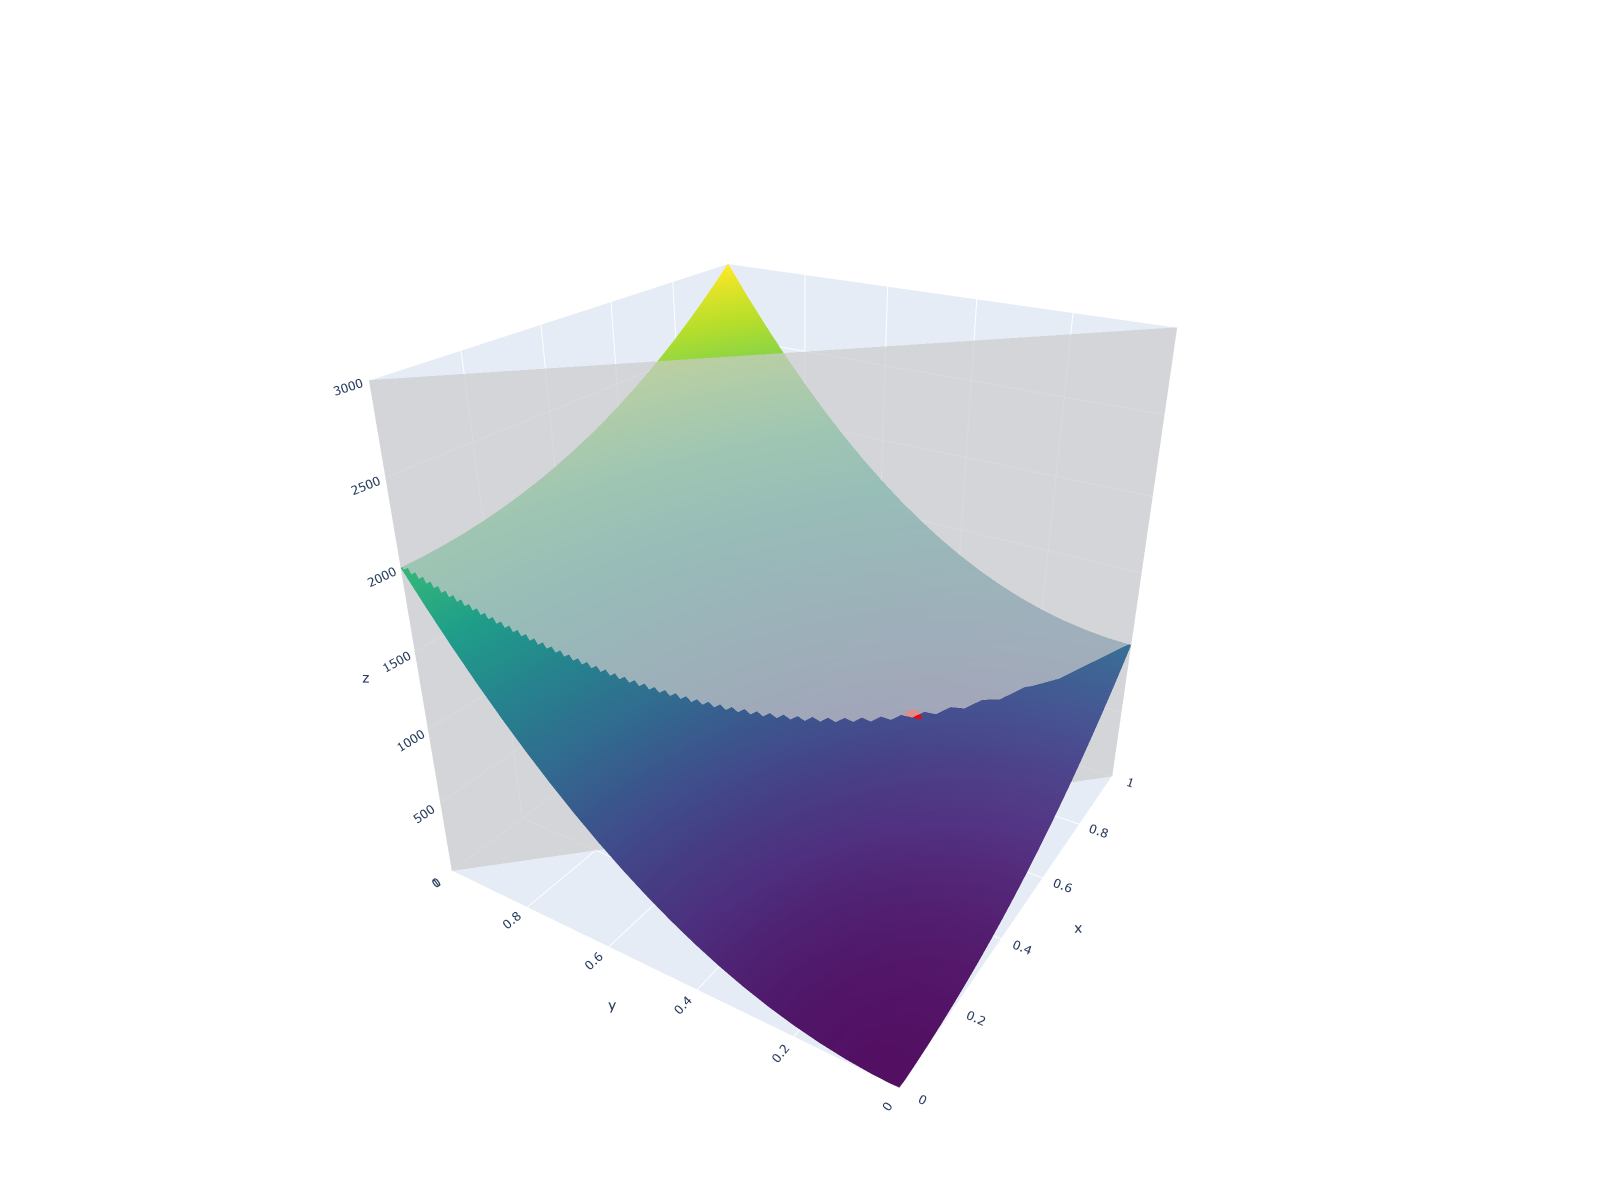
\includegraphics[width= 0.8\linewidth]{01_Pictures/newplot.png}
	\end{figure}
%	\begin{equation}
%		\textcolor{orange}{\frac{\partial F}{\partial z}(x, y, \phi, \frac{\partial \phi}{\partial x}, \frac{\partial \phi}{\partial y})}-\textcolor{brown}{\frac{\partial}{\partial x} \frac{\partial F}{\partial z_x}(x, y, \phi, \frac{\partial \phi}{\partial x}, \frac{\partial \phi}{\partial y})}-\textcolor{violet}{\frac{\partial}{\partial y} \frac{\partial F}{\partial z_y}(x, y, \phi, \frac{\partial \phi}{\partial x}, \frac{\partial \phi}{\partial y})}=0
%		\label{circuit:euler_lagransky}
%	\end{equation}

\end{frame}


%\begin{frame}
%	\frametitle{Lagrange Funktion finden}
%	% wir können nun die vorherigen gleichungen nehmen und einsetzen
%	
%	\begin{equation}
%		\nabla(\sigma \nabla \phi)=0
%		\label{circuit:current_density_5}
%	\end{equation}
%	\begin{equation}
%		\nabla^2 \phi=0
%		\label{circuit:current_density_6}
%	\end{equation}
%	\begin{equation}
%		P=\int_V \sigma(\nabla \phi)^2 d V
%		\label{circuit:current_density_7}
%	\end{equation}
%	\begin{itemize}
%		\item Kirchhoffsche Regel
%		\item Lagrange Funktion finden
%		\item Lagrange Funktion lösen 5. Schritte
%		\item Konkretisieren
%		\item Implementieren
%		\item Verstehen
%		\item Fragen
%	\end{itemize}
%\end{frame}
\section{Lagrange Funktion lösen}
\begin{frame}
	\frametitle{Lagrange Funktion lösen}
	\begin{enumerate}
		%		\item abc
		\item<1-> Schritt: Lagrange-Funktion des Problems ohne $\sigma$
		\begin{equation}
			L(x, U, U_x)= U_x^2 = \left(U_{x_1}^2+U_{x_2}^2\right)
		\end{equation}
		\item<2-> Schritt: partielle Ableitungen
		\begin{equation}
			\begin{aligned}
				\frac{\partial L}{\partial U}=0\\
				\frac{\partial L}{\partial U_{x_1}}=2U_{x_1}\\
				\frac{\partial L}{\partial U_{x_2}}=2U_{x_2}\\
			\end{aligned}
		\end{equation}
		\item<3-> Schritt: Ableiten nach $x_1$ und $x_2$
		\begin{equation}
			\begin{aligned}
				\frac{\partial L}{\partial U_{x_1}}(x,\phi,\nabla \phi)=2\frac{\partial \phi}{\partial {x_1}}\\
				\frac{\partial L}{\partial U_{x_2}}(x,\phi,\nabla \phi)=2\frac{\partial \phi}{\partial {x_2}}\\
			\end{aligned}
		\end{equation}
%		\item<4-> Schritt: Euler-Ostrogradsky Differentialgleichung
%		\begin{equation}
%			-\frac{\partial}{\partial x_1}\cdot 2\frac{\partial \phi}{\partial {x_1}}-\frac{\partial}{\partial x_2}\cdot 2\frac{\partial \phi}{\partial {x_2}}=-2\Delta\phi
%		\end{equation}
%		\item<5-> Schritt: Mögliche Lösungen
%		\begin{equation}
%			\sigma \cdot 2\Delta\phi=0
%		\end{equation}
%		Wir können nun noch durch $2\sigma$ teilen und bekommen die Laplace Gleichung.
%		\begin{equation}
%			\Delta\phi=0=\frac{\delta^2\phi}{\delta x^2}+\frac{\delta^2\phi}{\delta y^2}
%			\label{circuit:laplace1}
%		\end{equation}
		%\begin{equation}
		%	\Delta \phi(x,y)=\frac{\delta^2\phi}{\delta x^2}+\frac{\delta^2\phi}{\delta y^2}=0
		%\end{equation}
	\end{enumerate}
\end{frame}


\begin{frame}
	\frametitle{Lagrange Funktion lösen}
	\begin{enumerate}
		\setcounter{enumi}{4}
		\item<1-> Schritt: Euler-Ostrogradsky Differentialgleichung
		\begin{equation}
			-\frac{\partial}{\partial x_1}\cdot 2\frac{\partial \phi}{\partial {x_1}}-\frac{\partial}{\partial x_2}\cdot 2\frac{\partial \phi}{\partial {x_2}}=-2\Delta\phi
		\end{equation}
		\item<2-> Schritt: Mögliche Lösungen
		\begin{equation}
			\sigma \cdot 2\Delta\phi=0
		\end{equation}
		\begin{equation}
			\Delta\phi=0=\frac{\delta^2\phi}{\delta x^2}+\frac{\delta^2\phi}{\delta y^2}
			\label{circuit:laplace1}
		\end{equation}
		%\begin{equation}
		%	\Delta \phi(x,y)=\frac{\delta^2\phi}{\delta x^2}+\frac{\delta^2\phi}{\delta y^2}=0
		%\end{equation}
	\end{enumerate}
\end{frame}
\section{Diskretisierung}
\begin{frame}
	\frametitle{Diskretisierung}
	\begin{equation}
		\begin{aligned}
			f^{\prime \prime}(x) \approx \frac{\delta_h^2[f](x)}{h^2}&=\frac{\frac{f(x+h)-f(x)}{h}-\frac{f(x)-f(x-h)}{h}}{h}\\
			&=\frac{f(x+h)-2 f(x)+f(x-h)}{h^2}
		\end{aligned}
		\label{circuit:second-order-central}
	\end{equation}
	\center
	\begin{equation}
	\resizebox{0.9\textwidth}{!}{
	$
		\frac{\phi(x_{i+1}, y_j) - 2\phi(x_i, y_j) + \phi(x_{i-1}, y_j)}{(\Delta x)^2} + \frac{\phi(x_i, y_{j+1}) - 2\phi(x_i, y_j) + \phi(x_i, y_{j-1})}{(\Delta y)^2} = 0
	$}
	\end{equation}
	\begin{equation}
		\phi(x_i, y_j) = \frac{1}{4}(\phi(x_{i+1}, y_{j}) + \phi(x_{i-1}, y_{j}) + \phi(x_{i}, y_{j+1}) + \phi(x_{i}, y_{j-1}))
	\end{equation}
	\begin{equation}
		\phi(x_i, y_j) \to \frac{1}{4}(\phi(x_{i+1}, y_{j}) + \phi(x_{i-1}, y_{j}) + \phi(x_{i}, y_{j+1}) + \phi(x_{i}, y_{j-1}))
	\end{equation}
\end{frame}

\section{Python}
\begin{frame}
	\frametitle{Python}
	\begin{figure}[h]
		\centering
		\begin{figure}
			\centering
			\subfloat[Potential Distribution\label{fig:c}]{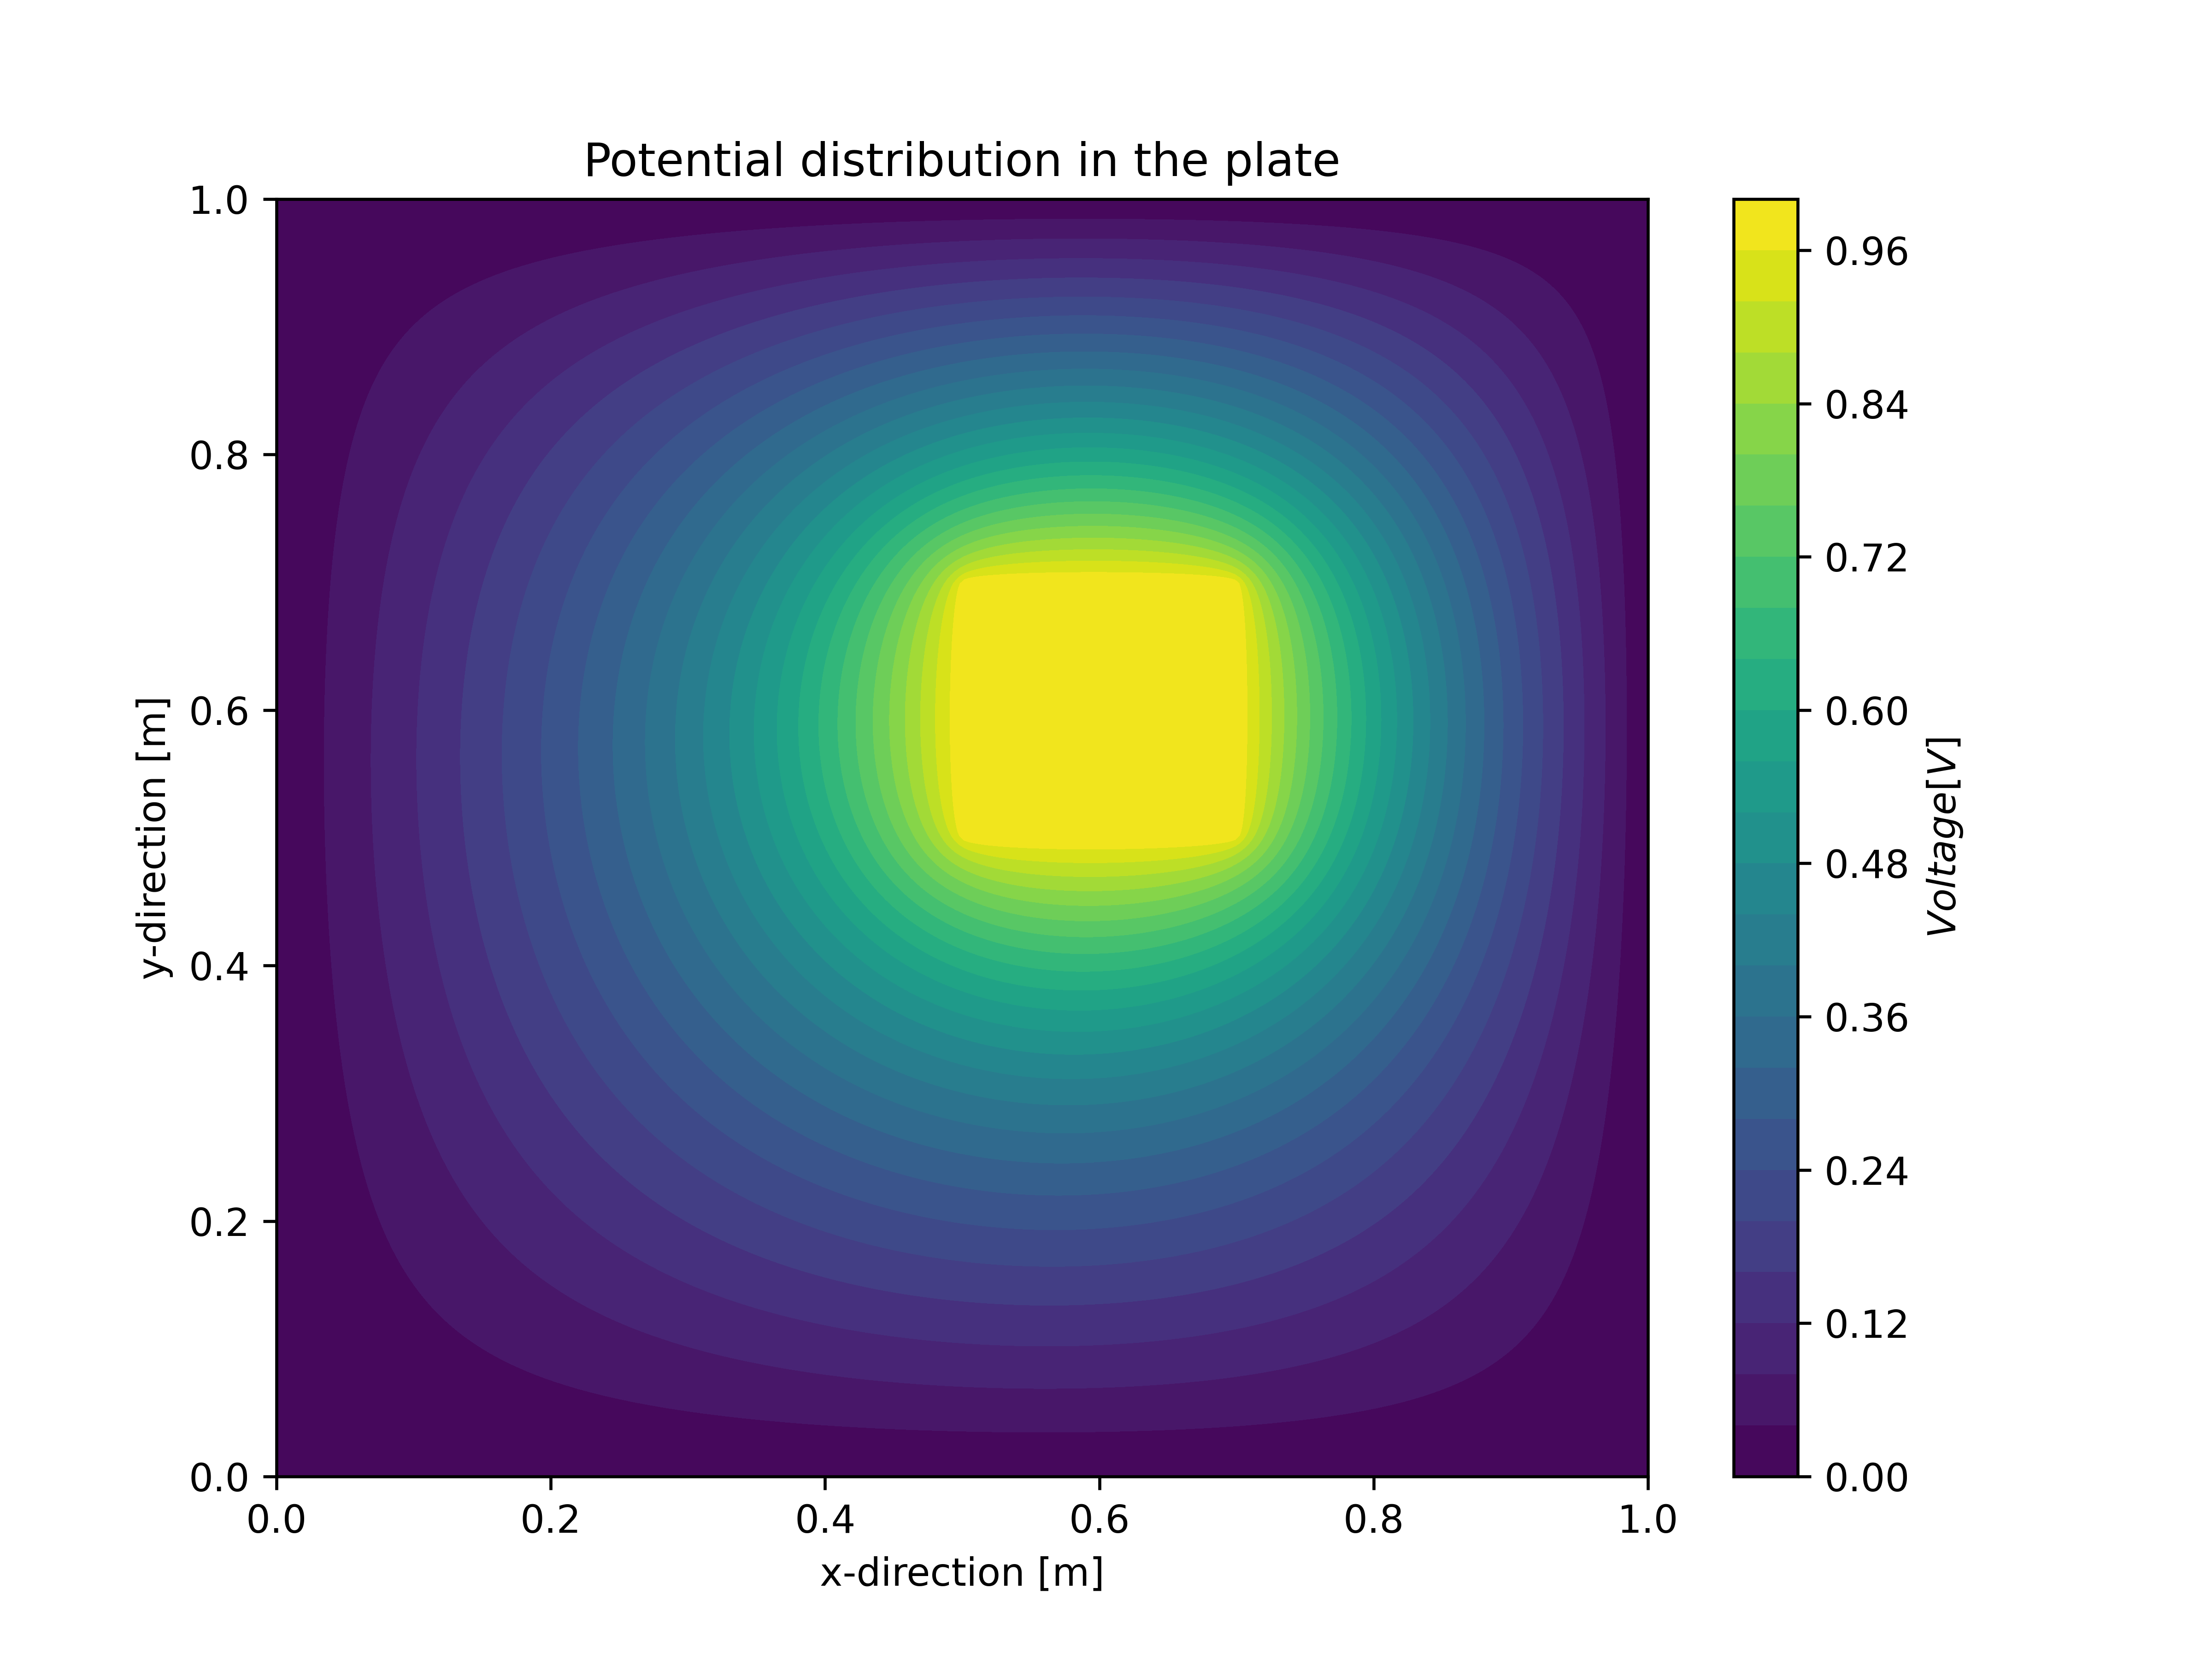
\includegraphics[width=0.45\textwidth]{01_Pictures/potential_distribution.png}}\qquad    
			\subfloat[Power Distribution\label{fig:d}]{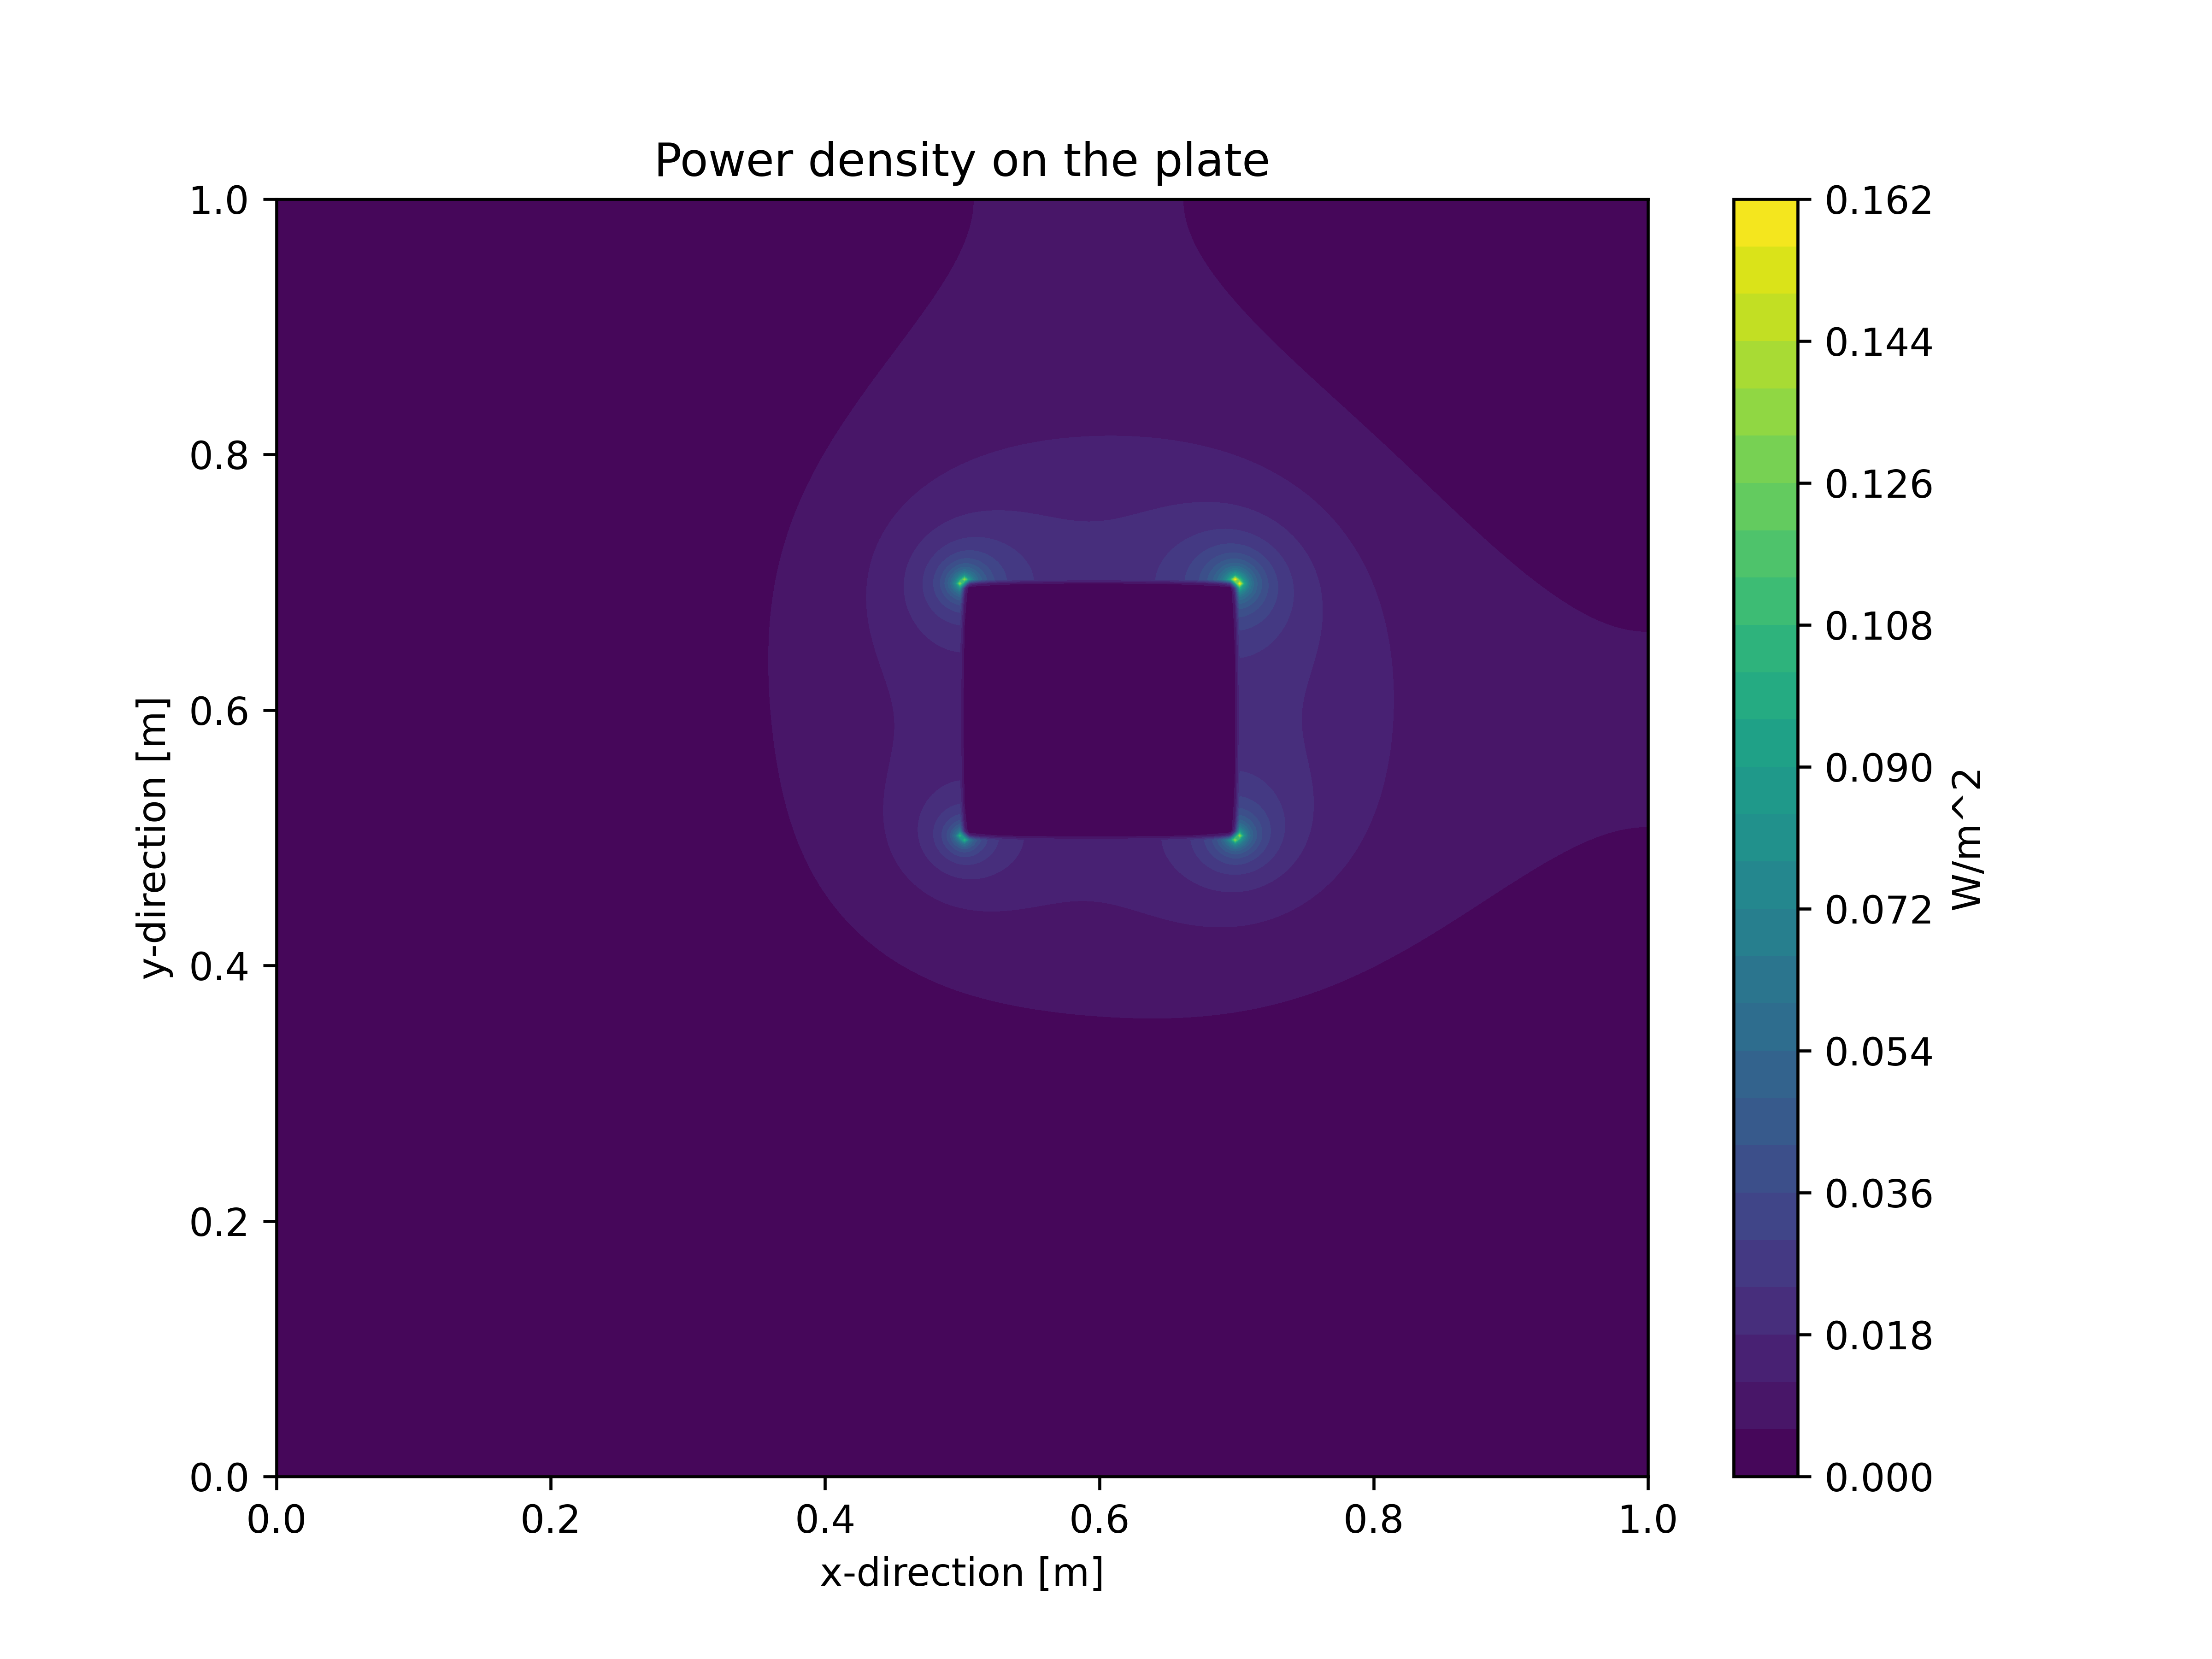
\includegraphics[width=0.45\textwidth]{01_Pictures/power_distribution.png}}
			\caption{Python Plots}
			\label{fig:2}
		\end{figure}
%		\begin{subfigure}[b]{0.3\textwidth}
%			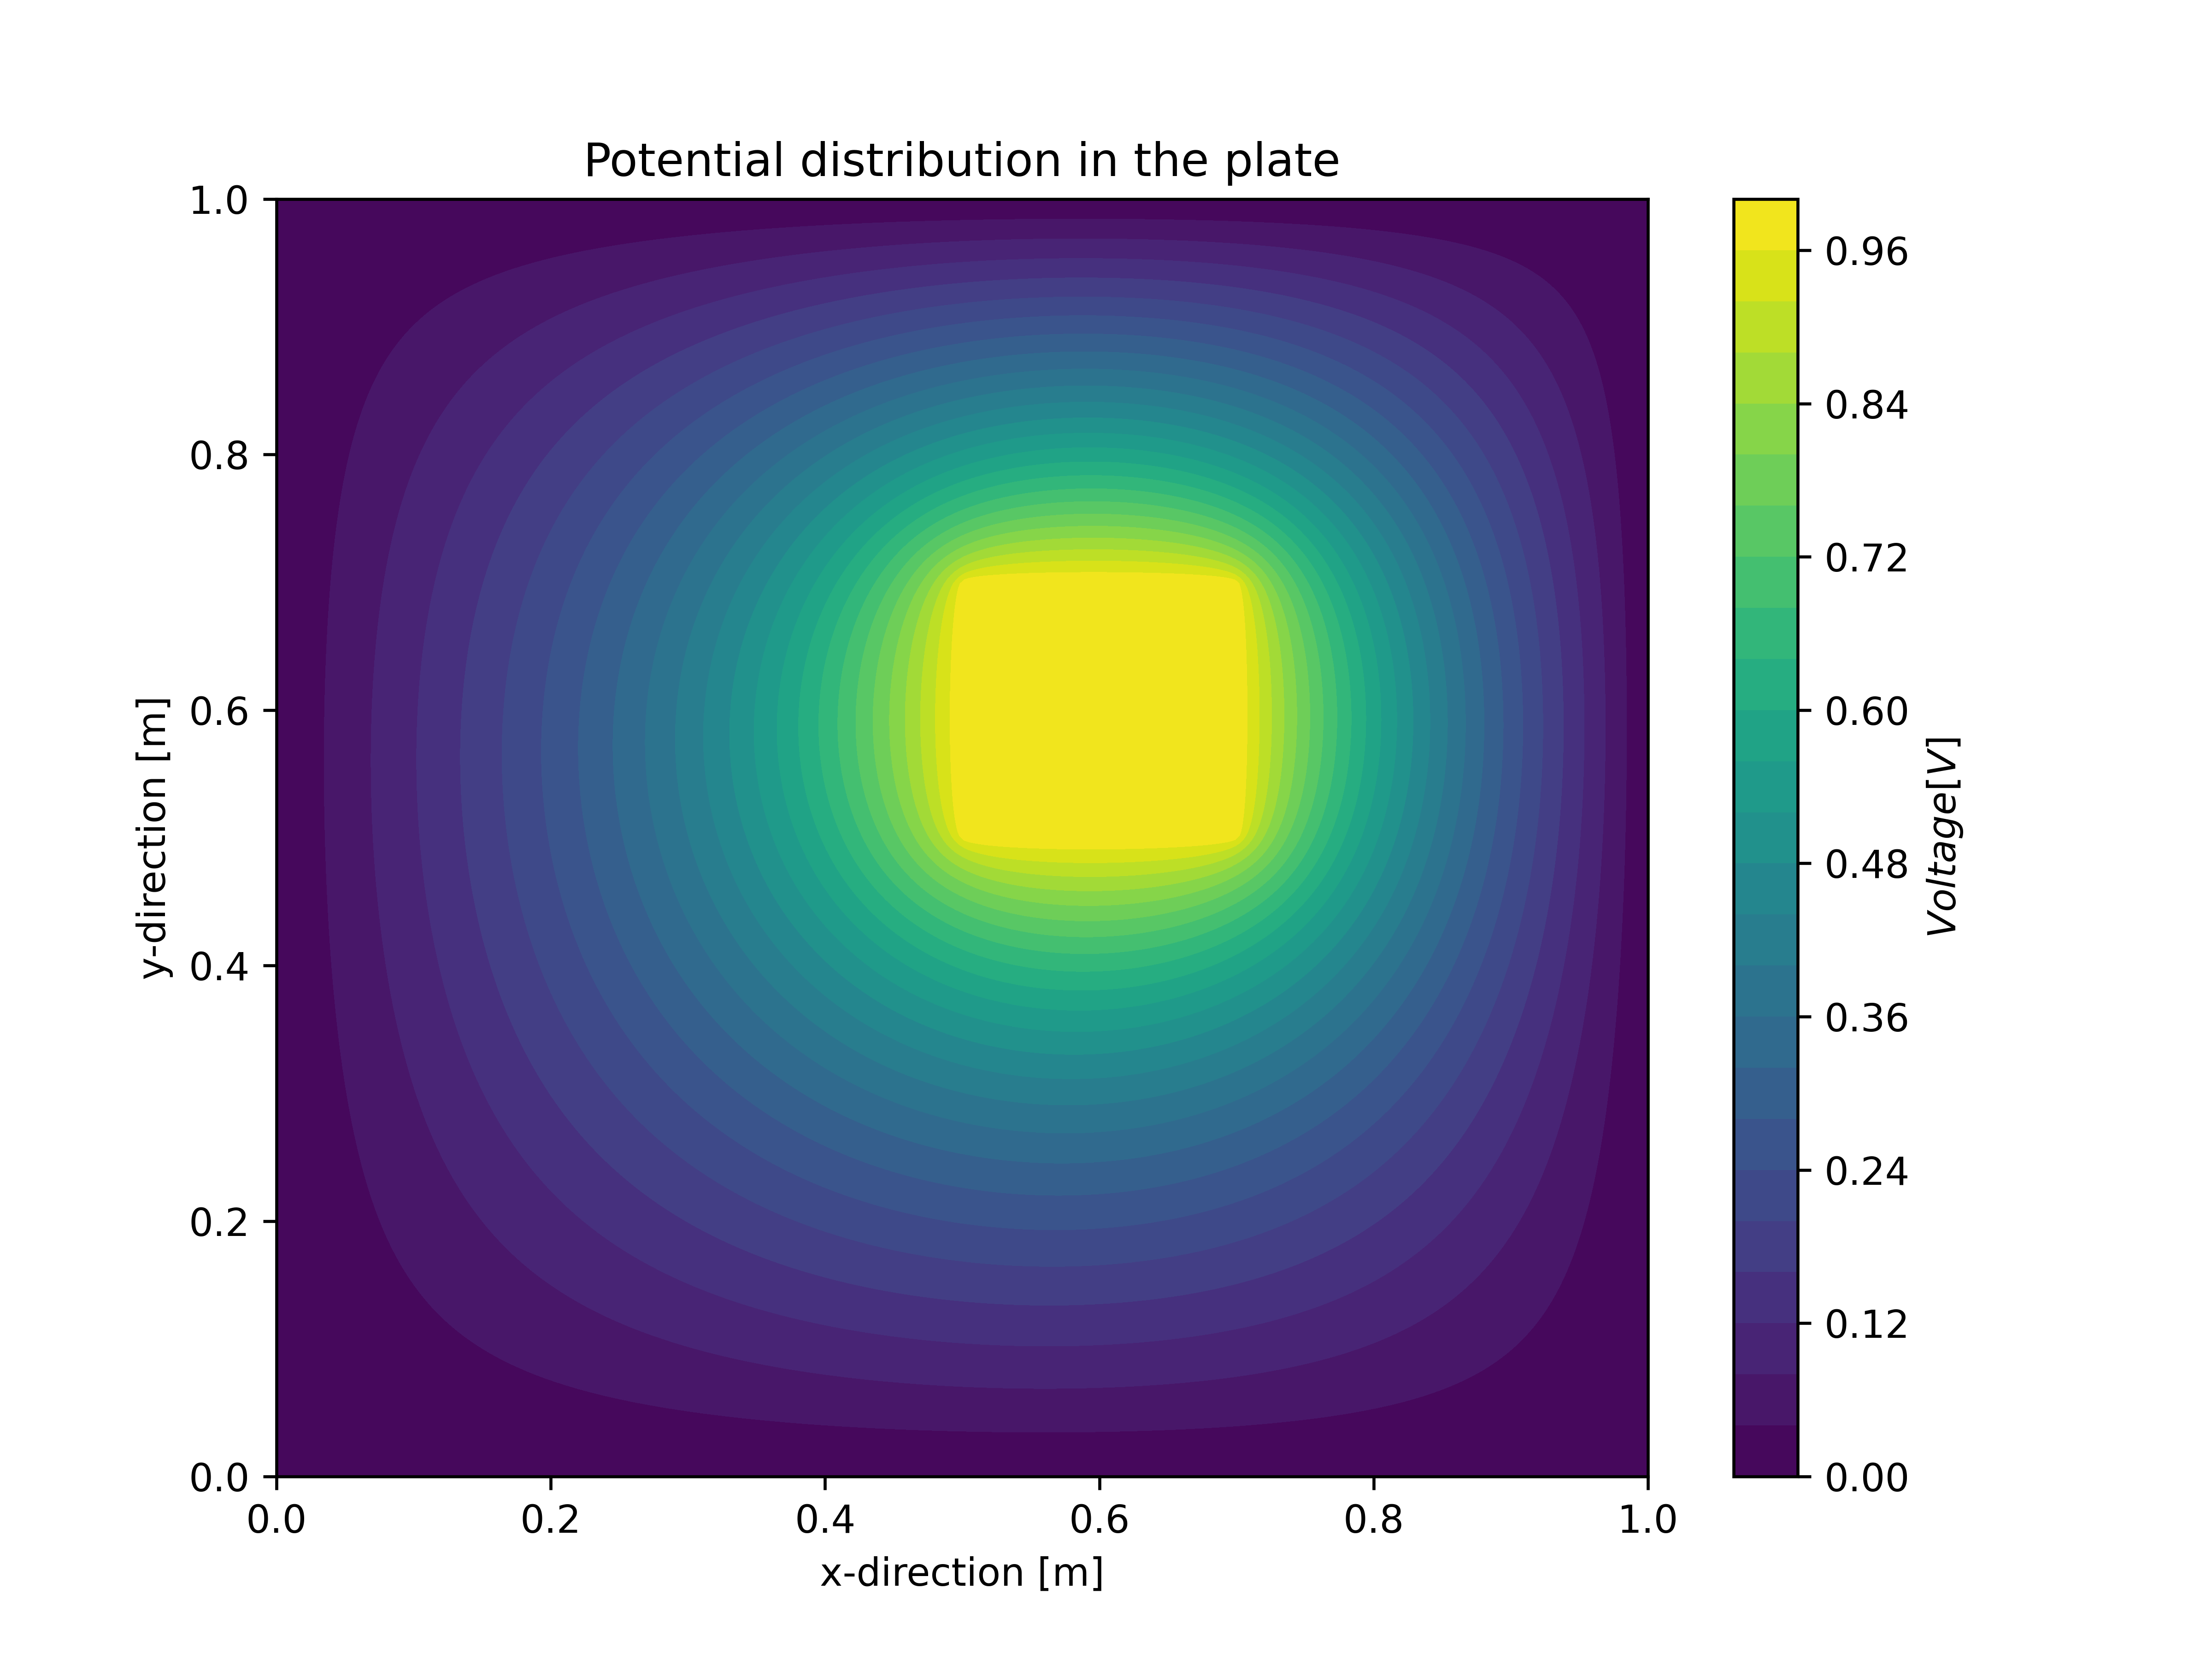
\includegraphics[width=\textwidth]{01_Pictures/potential_distribution.png}
%			\caption{Potential Distribution}
%			\label{fig:potential_distribution}
%		\end{subfigure}
%		\hfill
%		\begin{subfigure}[b]{0.3\textwidth}
%			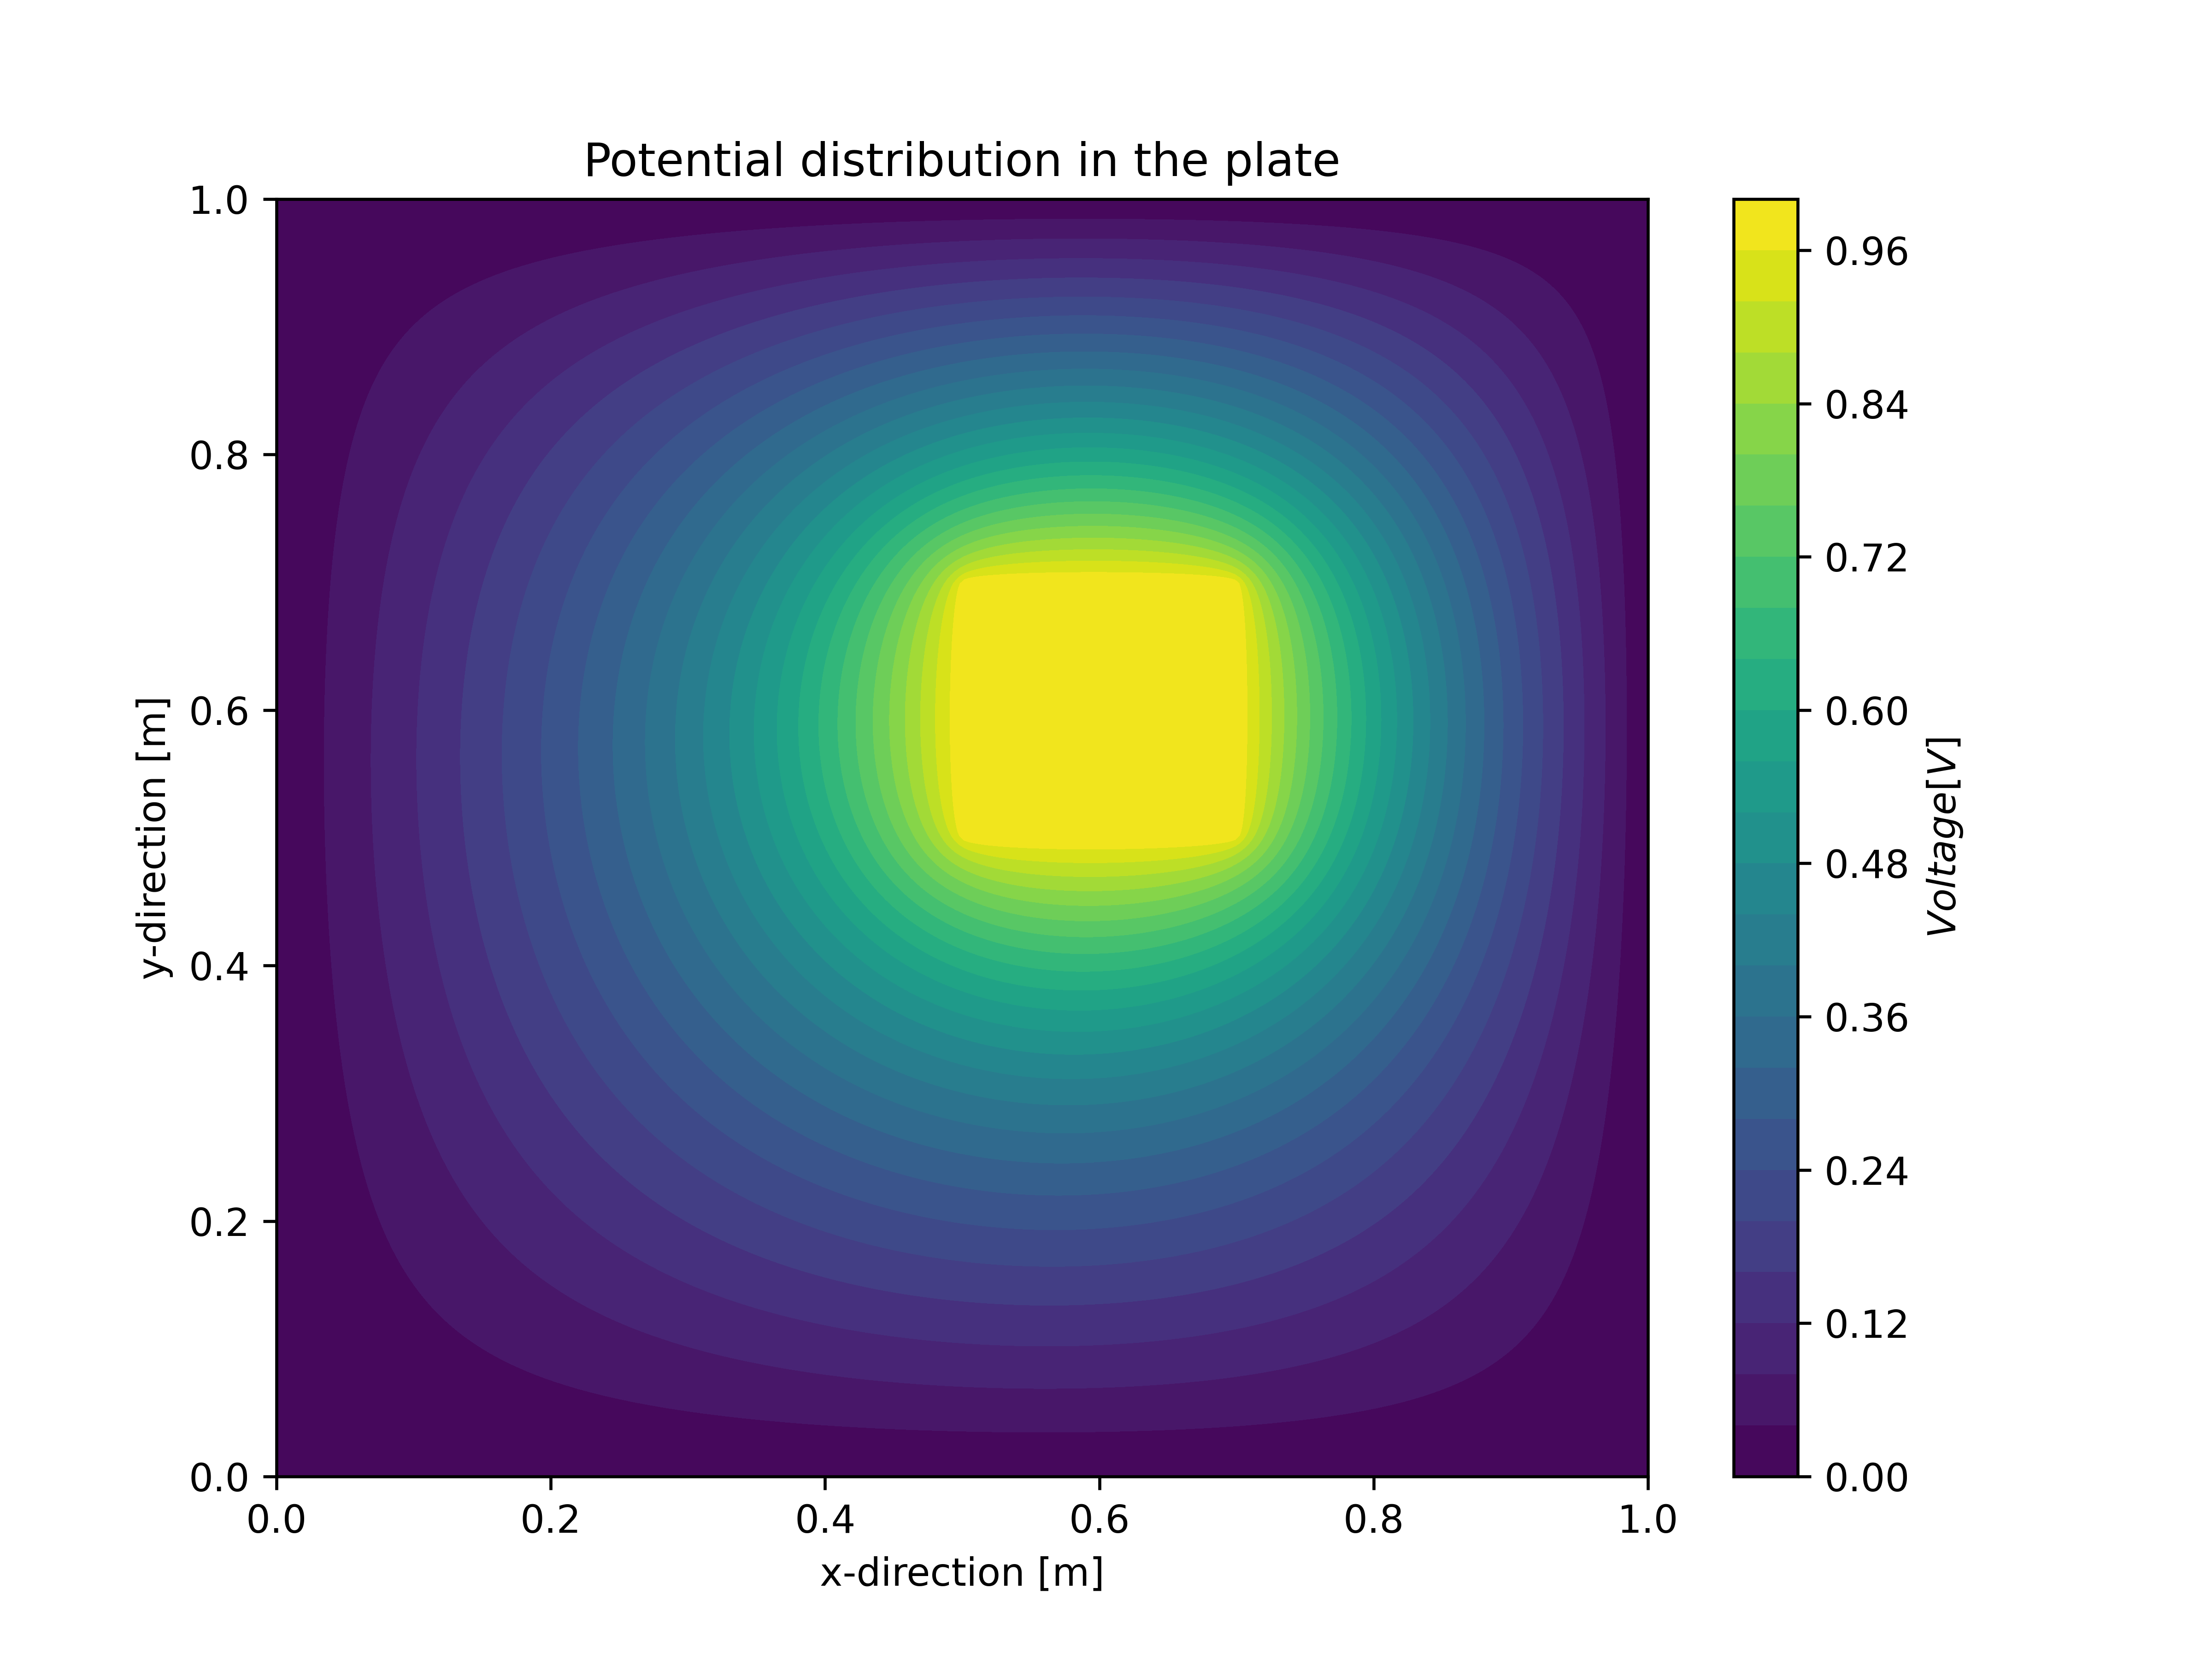
\includegraphics[width=\textwidth]{01_Pictures/potential_distribution.png}
%			\caption{Power Distribution}
%			\label{fig:power_distribution}
%		\end{subfigure}
%		\hfill
%		\begin{subfigure}[b]{0.3\textwidth}
%			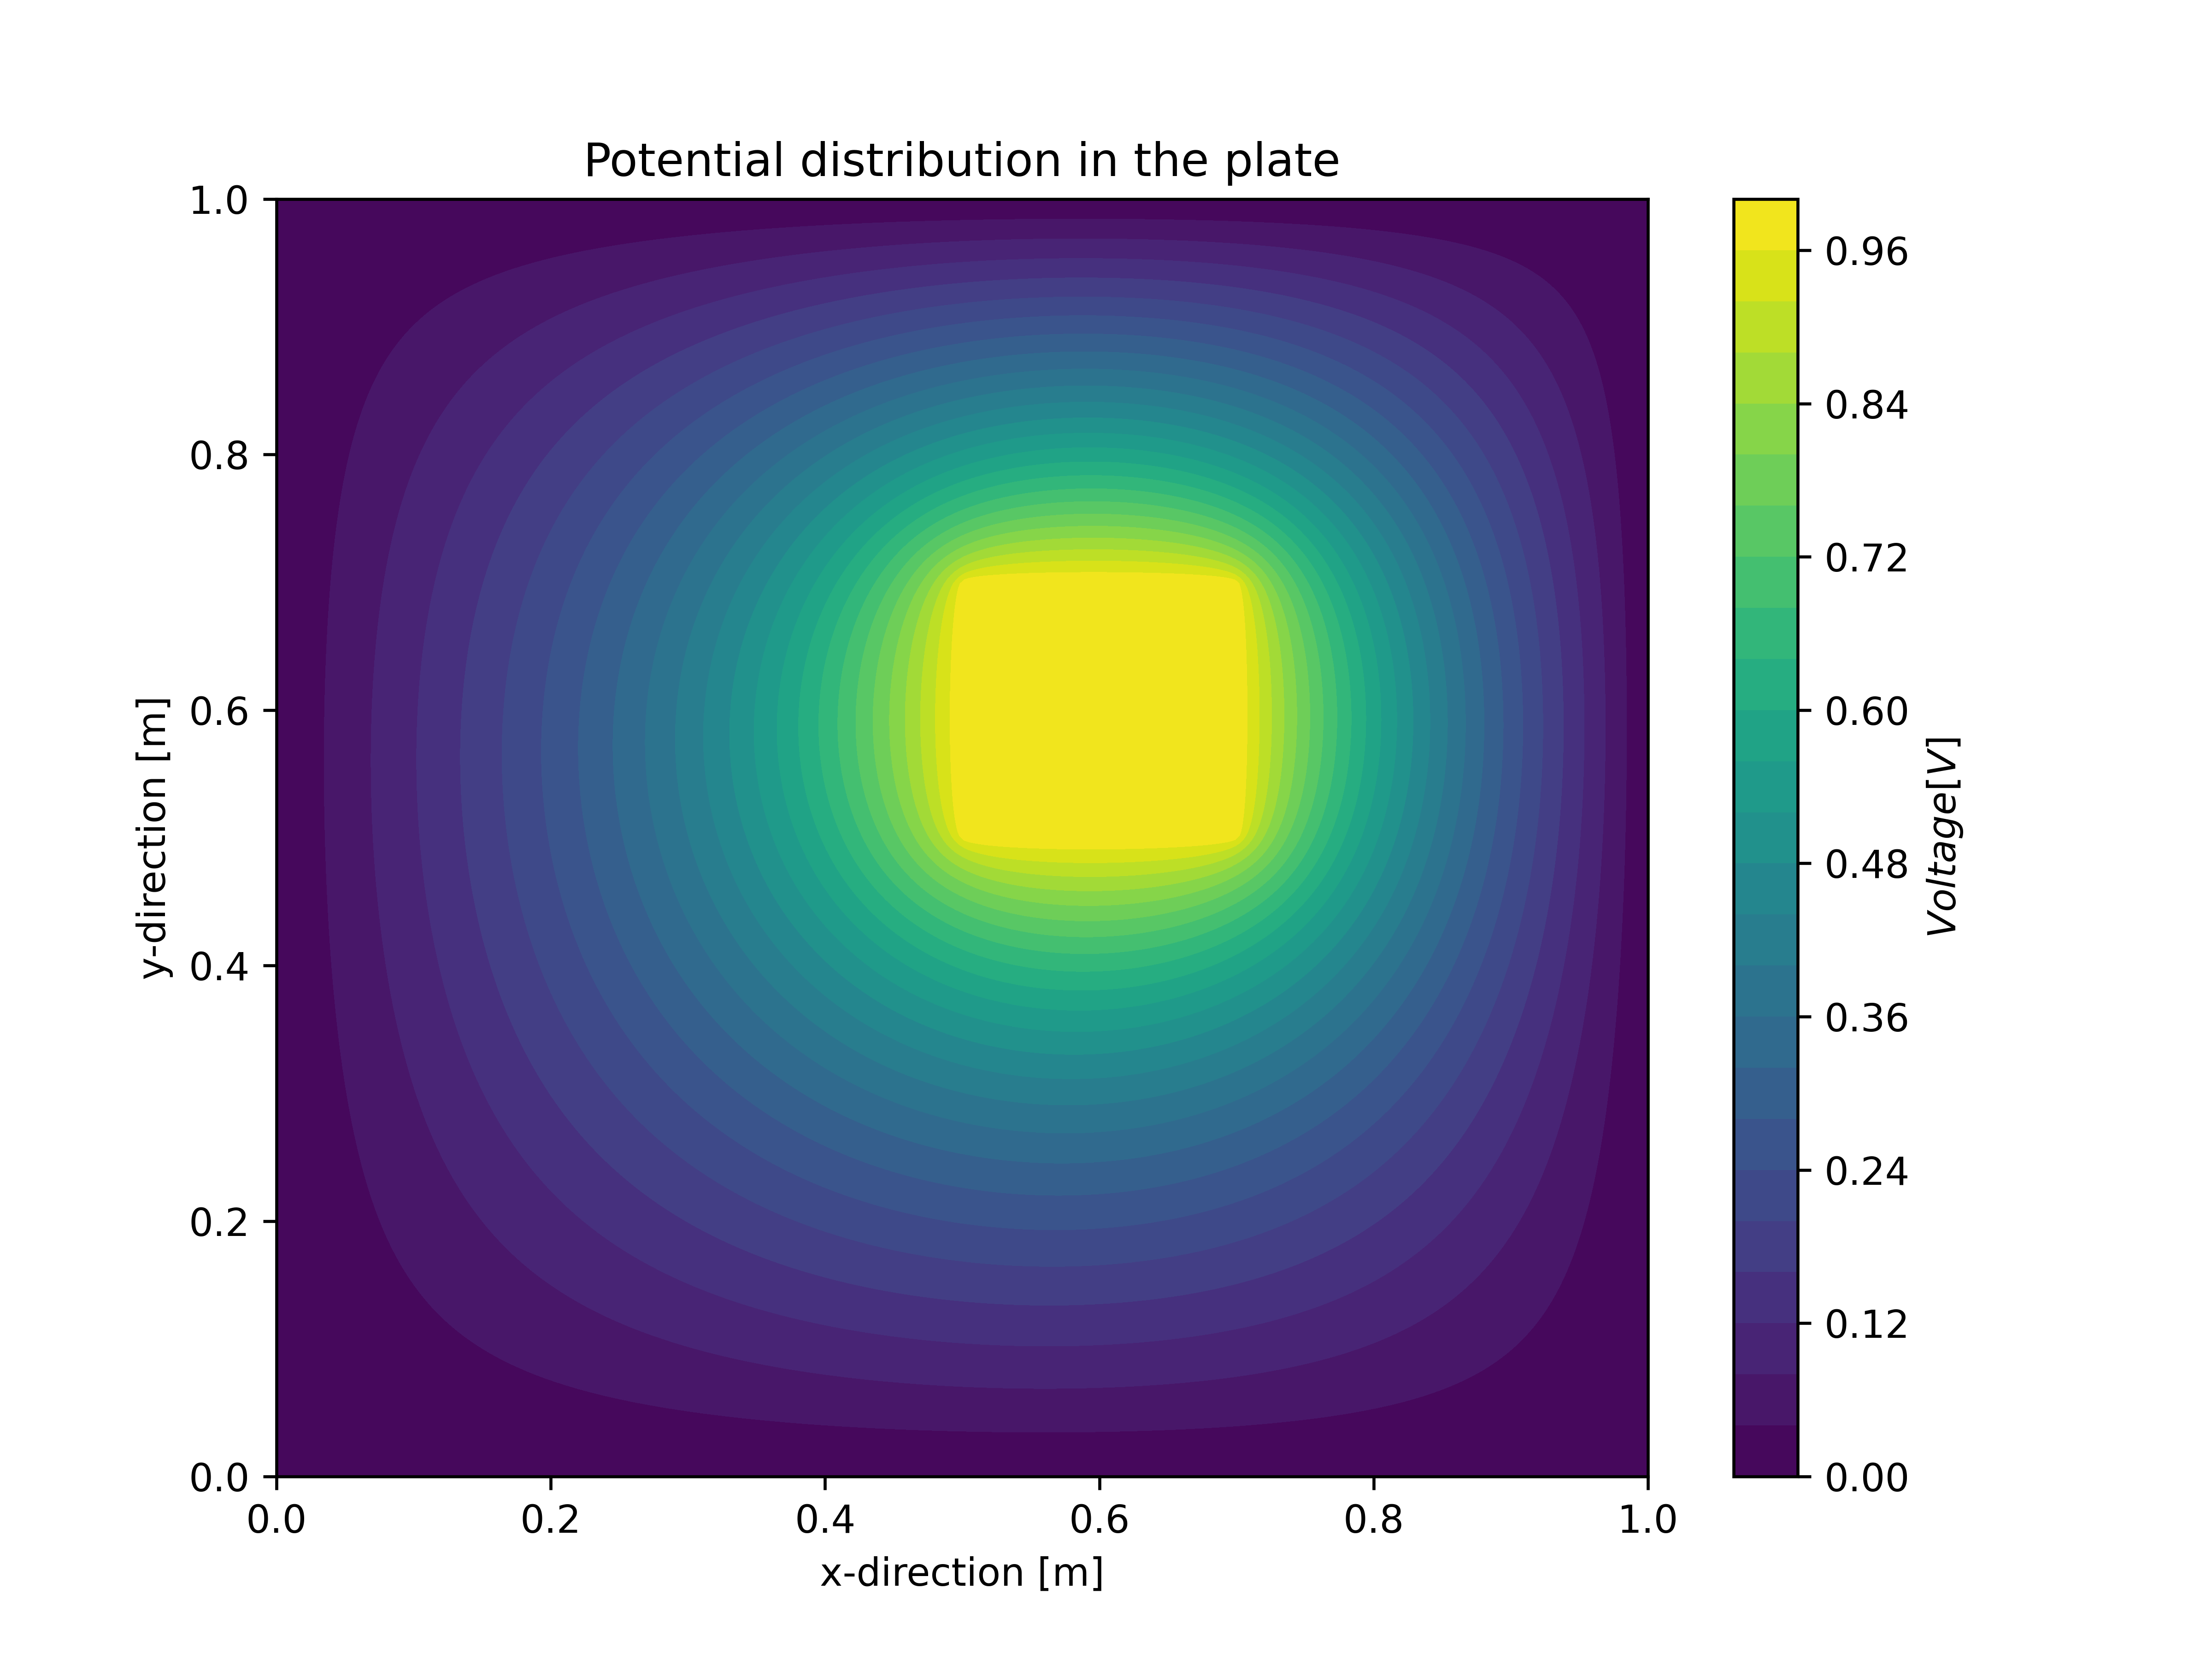
\includegraphics[width=\textwidth]{01_Pictures/potential_distribution.png}
%			\caption{Two Parallel Resistors}
%			\label{fig:two_parallel_resistors}
%		\end{subfigure}
%		\caption{Three subfigures showing the potential distribution, power distribution, and two parallel resistors.}
%		\label{fig:three_subfigures}
	\end{figure}
\end{frame}

\section{Fragen}
\begin{frame}
	\frametitle{Fragen}
	\begin{figure}
		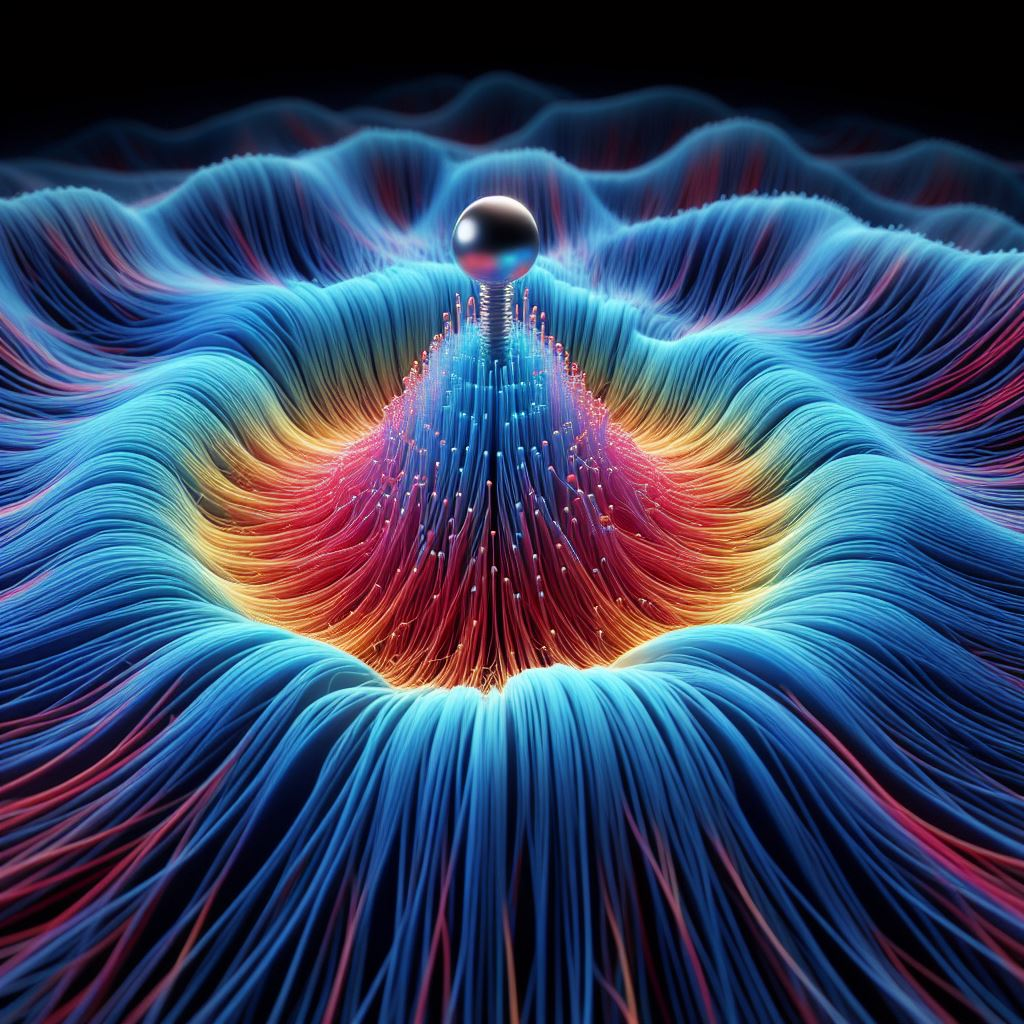
\includegraphics[width= 0.5\linewidth]{01_Pictures/ai.jpeg}
		\caption{AI potential plot, created with copilot}
	\end{figure}
\end{frame}




\end{document}
